\documentclass[../main.tex]{subfiles}
	% THE RASPBERRY PI AND THE TEST BED
\begin{document}

The communications test bed consists of a transmitter and a receiver Raspberry Pi, and a number of custom chips arranged on prototyping breadboards.
This section details the physical set-up of the test bed, the Raspberry Pi interface and the installation of the custom libraries used.
It also covers the technical specifications of the components and the details of the software underlying its operation.

%%%%%%%%%%%%%%%%%%%%%%%%%%%%%%%%%%%%%%%%%%%%%%%%%%%%%%%%%%%%%%%%%%%%%%%%%%%%%%%%%%%%%%%%%%%%%%%%%%%%%%%%%%%%%%%%%%%%%%%%%%%%%%%%%%

\section{Raspberry Pi Fundamentals}

The Raspberry Pi is a small, simple and affordable ARM-based computing module (Figure \ref{fig_Raspberry Pi}).
It has General Purpose Input/Output (GPIO) pins which it can use to interface with external peripherals.
The GPIOs can only take binary values of '0' (\SI{0}{\volt}) or '1' ($V_{max} = 3.3V$), and so converters are needed to output or input analogue signals.
The Pi is run on a Linux-based operating system called Raspbian, which is available for download from the Raspberry Pi official website
\cite{lib_Raspbian}.\\

\begin{figure}[ht]
	\centering
	\includegraphics[width=0.8\textwidth]{Raspberry_Pi.jpg}
	\caption{The Raspberry Pi with its case, a prototyping breadboard and some jumper cables}
	\label{fig_Raspberry Pi}
\end{figure}

The Raspberry Pi 3 Model B+ which is used for this project has a \SI{1.4}{\giga\hertz} 64-bit quad-core processor.
The main chip on the board is the Broadcom BCM2835.
The Pi's pins can either be numbered sequentially as pins 1 through 40 down the board - this is the BOARD numbering scheme, or they can be referred to by their Broadcom pin numbers - the BCM numbering scheme.
The second scheme numbers the available GPIO pins in the range 2-27 (Pins 0 and 1 are reserved for system use), where the rest of pins are not assigned numbers as they are power or ground pins.

\subsection{Setting up the Raspberry Pi}

\lstset{style=python}
The Raspberry Pi can be interfaced with in a number of ways, but first it needs to be set up with its operating system on the SD card \cite{web_SetupRaspbian}.
Raspbian can be controlled via the Command Line Interface (CLI) - typing in commands - or through an X Window graphical user interface (GUI) similar to Windows Operating System.
Either of these options can be used by connecting a screen, keyboard and mouse to the Pi, but this is not always available.
Alternative remote acess is possible using Secure Shell (SSH) set up for the command line, or Virtual Network Computing (VNC) for the X Window interface.
Secure Shell is necessary in this case, as it is used in the test bed execution.
When actually using the test bed, both Raspberry Pis are run in command line mode as this saves resources, although during development, VNC or a screen using the X Window makes it much easier to test and edit code.
In the test bed, the transmitter Pi is connected to a screen and keyboard, and then it starts the receiver via SSH, which runs headless (without a screen or control peripherals) and receives the data, processes and outputs it, and stores information about the run in a log file which can be accessed later or again through SSH.\\

\begin{figure}[ht]
	\centering
	\includegraphics[width=0.8\textwidth]{RPi_Setup.png}
	\caption{The setup procedure of the Raspberry Pi}
	\label{fig_RPi Setup}
\end{figure}

The setup procedure is shown in Figure \ref{fig_RPi Setup}.
Once the operating system is written to the SD card, SSH can be enabled by creating an empty file \textit{ssh} in the main portion of the card before putting it in the Raspberry Pi (for setup using a screen and peripherals, this can be turned on in the configuration settings).
Now an Ethernet cable can be connected from a computer to the Pi and it can be logged into.
A program such as PuTTY for Windows can be used \cite{lib_PuTTY}, with \textit{pi@raspberrypi.local} as the host name so the IP address is not needed.
The standard login is \textit{username: pi} and \textit{password: raspberry}.
The command \colorbox{backcolour}{\lstinline{sudo raspi-config}} accesses the configuration settings where the file system can be expanded to the whole SD card, and other utilities such as Wi-Fi and VNC can be turned on.
Again, all utilities except for SSH should be turned off when using the final test bed to improve performance of the devices.
Once the Pi is connected to Wi-Fi and the IP address is known, it can be accessed remotely via the free RealVNC VNC Viewer and the X Window can be started with the command \colorbox{backcolour}{\lstinline{startx}} if it is not already set to open the X Window on startup in the configuration settings \cite{lib_RealVNCViewer}.
This access can be made permanent by setting the Pi to have a static IP address or with a free RealVNC account which lets it be accessed independent of the IP address.\\

With full control of the Pi, all that is needed is to download all of the libraries and software used by the test bed and clone the GitHub repository with its code.
The Python version used is 3.5.3. and as the Raspberry Pi has Python 2 and Python 3, \colorbox{backcolour}{\lstinline{pip}} - the Python package manager - is run as \colorbox{backcolour}{\lstinline{pip3}} for Python 3.
Any dependencies not in this list give clear instructions in the terminal as to how they are downloaded when this list is run line by line.\\

\begin{lstlisting}[caption=Libraries and Packages Required for the Test Bed,basicstyle=\footnotesize]
	sudo apt-get update
	
	sudo apt-get install vpnc
	sudo apt-get install libffi6 libffi-dev python-dev
	sudo pip3 install cryptography paramiko
	
	sudo apt-get install libatlas-base-dev
	sudo pip3 install numpy imageio
	sudo pip3 install matplotlib
	sudo apt-get install pigpio
	
	sudo apt-get install git
	cd "<Path for the code e.g. /pi/home/Documents/>"
	git clone https://github.com/CamEadie/4YP_PiCom

	sudo apt-get update && sudo apt-get upgrade && sudo apt-get dist-upgrade

	# Used in Transmit_Binary_Data(): import RPi.GPIO as GPIO
	# ... This library is already included in the Raspberry Pi
	# ... Only for OOK transmission which uses Python not C
	# Used in Check_Input_Masks(): from RPiSim.GPIO import GPIO
	# ... pip GPIOSimulator (or pip3 if necessary)
	# ... Only works in Windows, simulates Raspberry Pi pins (use like RPi.GPIO commands)
\end{lstlisting}

Included are the following, as well as their dependencies:\\

\begin{itemize}
	\item \textit{VPNC} - VPN software used to access Oxford VPN in order to use the OWL Wi-Fi network \cite{lib_VPNC}
	\item \textit{Paramiko} - Python library used for SSH to start the receiver \cite{lib_Paramiko}
	\item \textit{NumPy} - Python library used for easier array manipulation as well as interface with images \cite{lib_NumPy}
	\item \textit{imageio} - Python library used to read and save image files as \textit{NumPy} arrays \cite{lib_imageio}
	\item \textit{matplotlib} - Python library used to plot graphs of data using a MATLAB-like interface \cite{lib_matplotlib}
	\item \textit{pigpio} - C library used to interface with the GPIO pins \cite{lib_pigpio}
	\item \textit{Git} - Version control software which also allows for the cloning of the project code to any device \cite{lib_Git}
\end{itemize}

%%%%%%%%%%%%%%%%%%%%%%%%%%%%%%%%%%%%%%%%%%%%%%%%%%%%%%%%%%%%%%%%%%%%%%%%%%%%%%%%%%%%%%%%%%%%%%%%%%%%%%%%%%%%%%%%%%%%%%%%%%%%%%%%%%
	
\section{Test Bed Architecture}

The test bed comprises the two Raspberry Pis and a number of chips to provide the functions required for more advanced modulation schemes.
This is built up as three arrangements with increasing complexity, eventually all integrated into the final setup.
The first is the Pis connected together by three wires, a serial data line, a clock line and a connection between ground pins as shown in Figure Figure \ref{fig_OOK Architecture}.
This arrangement is similar to that used for the Inter-Integrated-Circuit ($I^2C$) bus, however the code written for this form of communication does not rely on any available modes of serial interfacing because it needs to be extensible to the parallel communication in the next arrangements.
The second arrangement is used for Pulse Amplitude Modulation schemes.
It uses a single parallel Digital Analogue Converter (DAC) connected to the transmitter which transmits to a parallel Analogue Digital Converter connected to the receiver, allowing for multi-level signals to be transmitted between the two devices (at baseband, this can also be modulated using the next setup).
The final arrangement extends the set-up to two DACs and two ADCs.
These signals are then modulated by a sine wave and a cosine wave respectively and added, and can be separated at the receiver due to the orthogonality of the two signals.
This arrangement is used for Quadrature Amplitude Modulation as well as Orthogonal Frequency Division Multiplexing.\\

\begin{figure}[ht]
	\centering
	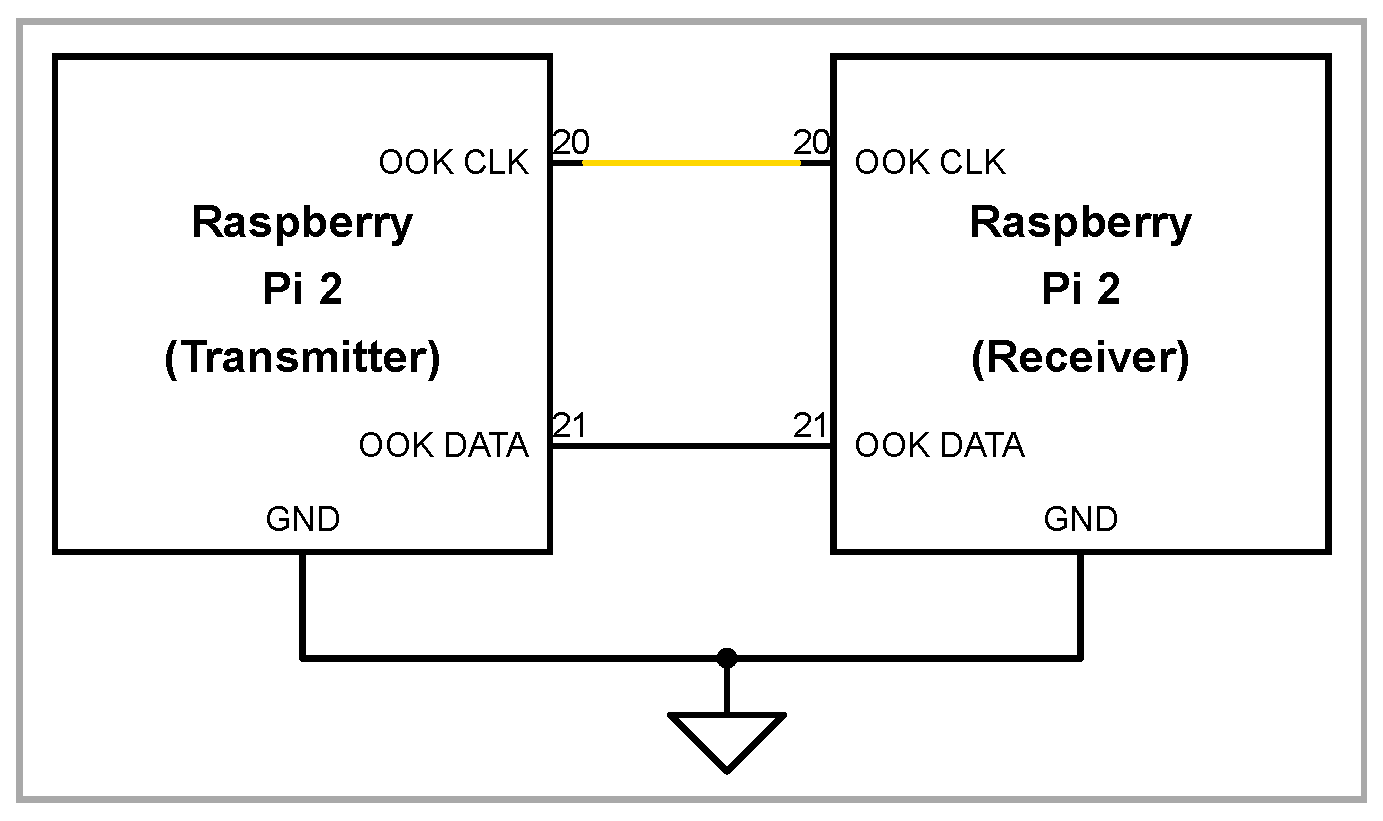
\includegraphics[width=0.6\textwidth]{ook_architecture.eps}
	\caption{Test Bed Set-up For On-Off Keying}
	\label{fig_OOK Architecture}
\end{figure}

\subsection{Digital Analogue Converter}

The Digital Analogue Converter (DAC) used is the AD5424, an 8-bit CMOS current output DAC with an easy interface to microcontrollers.
It has a \SI{17}{\nano\second} write cycle and a maximum update rate of \SI{20.4}{MSPS}. % Mega Samples Per Second
A parallel 8-bit DAC and equivalent Analogue Digital Converter (ADC) were chosen because they can achieve significantly higher data rates than a serial interface device which must transmit all eight bits per sample from one GPIO pin.
There are possible configurations in the data sheet using an inverting operational amplifier to produce the output, however due to the single supply and difficulties finding low-power operational amplifiers which provide rail-to-rail output for a 5V single supply, this was avoided where the output through a load resistor could produce the required voltages.
The Read/Write ($R/\overline{W}$) pin is pulled low so the chip is permanently in write mode; read back of the parallel digital outputs is not required.
The Chip Select pin ($\overline{CS}$) needs a falling edge and a rising edge to complete a write cycle.
This is because the DAC has a latched interface; the rising edge loads the new parallel data to be held in the latches and immediately provide the analogue output.
However, the latches are not transparent (the input is not visible while $\overline{CS}$ is low and the chip is selected), and so the output holds the analogue conversion of the latched digital byte only until the falling edge of $\overline{CS}$.
This pin is therefore connected to the clock pin of the Raspberry Pi, and the shape of the clock signal used to best utilise the DAC is discussed in Section \ref{sec_Advanced Modulation Schemes}.
The same clock pulses are also fed to the $\overline{WR}$ (start conversion) pin of the ADC.
Connections between the transmitter Raspberry Pi and the DAC are in Figure \ref{fig_DAC Layout}.\\

\begin{figure}[ht]
	\centering
	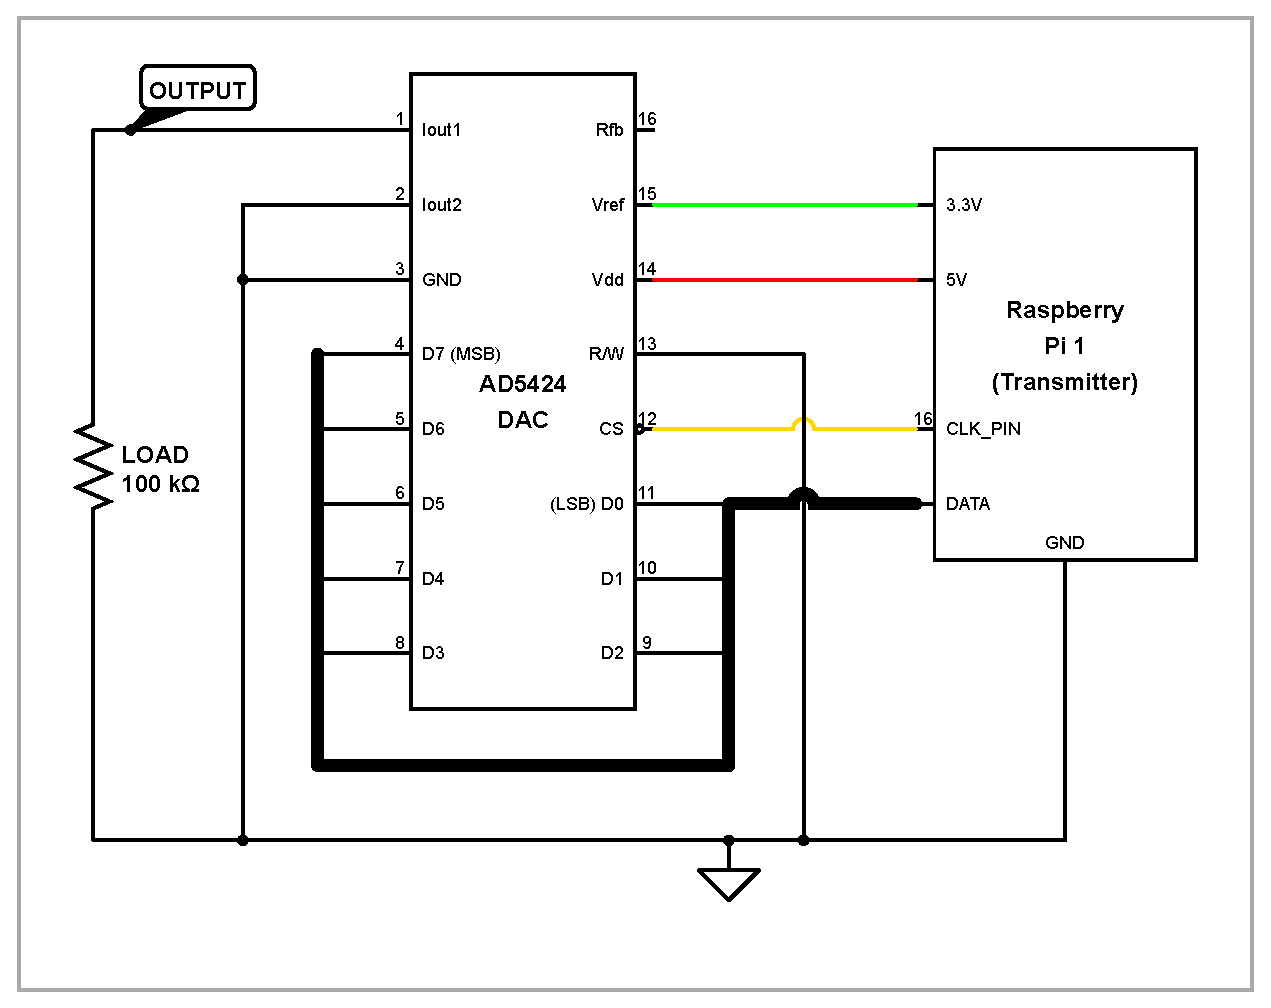
\includegraphics[width=0.8\textwidth]{ad5424.eps}
	\caption{Layout of the Digital Analogue Converter}
	\label{fig_DAC Layout}
\end{figure}

\subsection{Analogue Digital Converter}

The Analogue Digital Converter used is the ZN448, an 8-bit successive approximation ADC designed to be easily interfaced to microprocessors.
It operates with an on-chip clock with capability to be overdriven, and has a \SI{9}{\micro\second} conversion time guarantee.
Figure \ref{fig_ADC Layout} is a diagram of the ADC connections to both Raspberry Pis.
The converter is cleared when the $\overline{WR}$ (start conversion) pin is pulled low.
On the rising edge of this pin, the comparison of $\frac{V_{REF}}{2}$ to the Most Significant Bit (MSB) set to '1' and all other bits set to '0' is made, and the conversion from analogue to digital values continues by successively setting the next bit, making a comparison and so on.
Therefore $\overline{WR}$ is fed from the clock line of the transmitter Raspberry Pi.
The $\overline{BUSY}$ (end of conversion) pin goes low when the a conversion starts ($\overline{WR}$ is pulled low), and goes high when the conversion is complete.
The positive edge of this signal is taken as the clock for the Receiver.
This is because there is some delay in the ADC's calculation of its digital value, but on the rising edge of $\overline{BUSY}$ the resulting digital value at the output is correct and stays correct until the next negative pulse on $\overline{WR}$.
This works as long as the transmitter is not transmitting so fast as to transmit the next value before the ADC can finish converting the last one.
The $\overline{RD}$ (output enable) pin is pulled low to allow permanent non-destructive readout of the digital output.\\

\begin{figure}[ht]
	\centering
	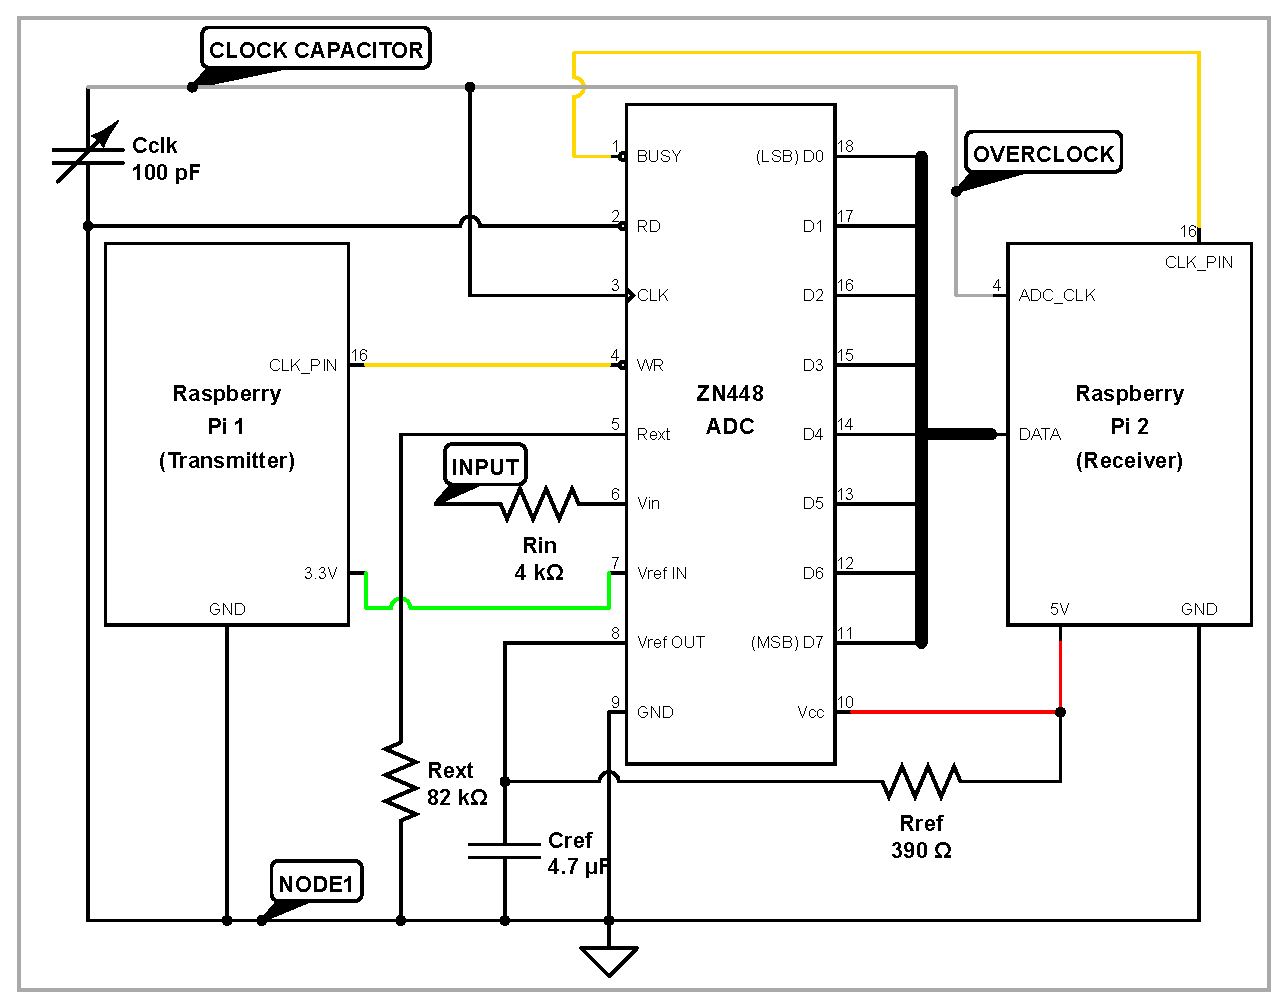
\includegraphics[width=0.8\textwidth]{zn448.eps}
	\caption{Layout of the Analogue Digital Converter}
	\label{fig_ADC Layout}
\end{figure}

The DAC's internal clock frequency is selected with the $CLK$ pin, either with a single clock capacitor (with an equivalent frequency table provided in the data sheet) or by providing an external clocking signal (see Section \ref{sec_Overclocking}).
Both options are shown as grey lines in the diagram and only one should be used.
The conversion by successive approximation works by approximating one bit per clock pulse over eight clock pulses.
The data sheet suggests that due to accepting a completely asynchronous convert pulse with respect to the clock, valid data is produced between 7.5 and 8.5 clock pulses later.
The maximum internal clock frequency is \SI{1}{\mega\hertz} and the guaranteed \SI{9}{\micro\second} conversion time (\SI{0.11}{MSPS}); a clock frequency giving 9 pulses between conversions is suggested to absolutely ensure complete conversion.
It is worth mentioning that although the maximum suggested capacitor-based or overdriving frequency of the internal clock is \SI{1}{\mega\hertz}, the data sheet states that all tests were done with an internal frequency of \SI{1.6}{\mega\hertz} suggesting this can be pushed.
The capacitor value of \SI{100}{\pico\farad} in Figure \ref{fig_ADC Layout} corresponds to a \SI{900}{\kilo\hertz} internal clock frequency, allowing for a sampling rate of at least \SI{0.1}{MSPS} % Mega Samples Per Second
(or equivalently a baud rate of at least \SI{100}{\kilo\hertz}) which is close to the extent of the converter.
Figure \ref{fig_PAM Architecture} is a picture of of the two Raspberry Pis connected together for baseband 4PAM communication.\\

\begin{figure}[ht]
	\centering
	\includegraphics[width=0.8\textwidth]{PAM_Architecture_Pic.jpg}
	\caption{Layout of Test Bed for Pulse Amplitude Modulation}
	\label{fig_PAM Architecture}
\end{figure}

\subsection{Quadrature Pulse Generator}

The pulse generator is the LTC-9608-2 which provides $90^o$ shifted (quadrature) output square waves.
The frequency is a function of a single setting resistor, with a value of $f_{out} = 10MHz \times \frac{10000}{R_{set}}$ and can operate up to \SI{10}{\mega\hertz}.
In order to produce sinusoidal output, a second order passive RC low-pass filter is used at each of the outputs.
One output is multiplied by the baseband signal for PAM modulation, and both are multiplied by the I and Q components of the output respectively and added together for QAM in order to quadrature-carrier modulate the signal.

\subsection{Multiplier} \label{sec_Multiplier}

The multiplier is the AD633, capable of four-quadrant multiplication and requiring no external components.
It also has a summing input, allowing the output of one multiplier to be added to the output of another.
The Pi is not able to output negative voltages.
As a result, Pulse Amplitude Modulation uses the range $0$ to $V_{max}$ rather than $-V_{max}$ to $V_{max}$.
Similarly, Quadrature Amplitude Modulation uses a grid of I and Q values all in the positive quadrant (0,1,2,3 not -3,-1,1,3).
The same "negative" effect is still achieved by using the "GROUND" of the multipliers (which are fully differential) as $V_{max/2}$ provided with a voltage divider.
This means that the sine and cosine signals would be inverted when multiplied by the values equating to 0 and 1 in the same way they would be for -3 and -1.
As a result the transmitted signal will be a regular PAM or QAM signal plus a DC component of $V_{max/2}$.
The final layout of the test bed is shown in Figure \ref{fig_QAM Layout}.

\begin{figure}[ht]
	\centering
	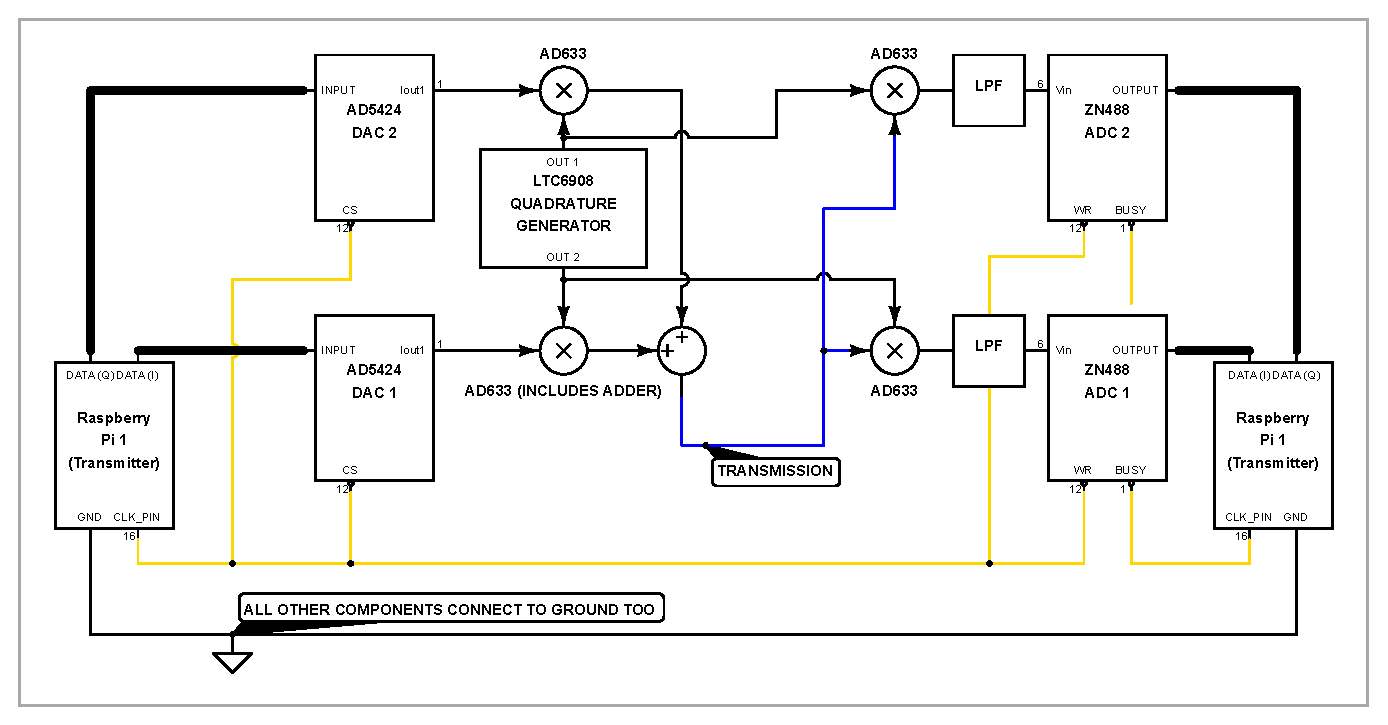
\includegraphics[width=\textwidth]{qam_archictecture.eps}
	\caption{Layout of the Test Bed for QAM and OFDM}
	\label{fig_QAM Layout}
\end{figure}

\subsection{Parts Used}

\begin{figure}[ht]
	\centering
	\includegraphics[width=0.3\textwidth]{DAC_Board.jpg}
	\includegraphics[width=0.3\textwidth]{ADC_Board.jpg}
	\includegraphics[width=0.3\textwidth]{ClockBoard.jpg}
	\caption{The DAC (left), DAC (centre) and Quadrature Pulse Generator (right) set-ups on individual breadboards}
	\label{fig_Breadboards}
\end{figure}

Figure \ref{fig_Breadboards} shows various chips and their on-board set-ups.
Table \ref{tab_Part Prices} is a table of all of the key parts used in the construction of the test bed, excluding small items such as resistors and capacitors.
The total retail price - without VAT (about $20\%$ on average) and handling charges of individual orders - comes to $\mathsterling$166.56.
Even with all of the additional components and charges this allows the test bed to be constructed for under $\mathsterling$250.
This is significantly cheaper than any of the examples considered in Section \ref{sec_Lit Review}.
This demonstrates that it is possible to construct a simple software-defined radio communications test bed using two Raspberry Pis at a much lower cost compared to purchasing or building a standard test bed architecture.
Although these more standard test beds may provide certain advanced capabilities, the key functionalities required should be achievable with this design.
The extent to which this architecture can successfully achieve these goals is a question investigated by the rest of the report.\\

\begin{table}[h]
	\centering
	\global\tabulinesep = 2mm
	\begin{tabu} to 0.8\textwidth { | X[l] | X[c] | X[c] | }
		\hline
		Component & Quantity & Price ($\mathsterling$)\\
		\hline\hline
		Raspberry Pi Model B+ + Case & 2 & 28.39 + 4.95\\
		\hline
		Breadboards + Jumper cables & -- & 21.96 + 11.05\\
		\hline
		DAC (AD5424) + Surface mount & 2 & 4.19 + 3.36\\
		\hline
		ADC (ZN488)  & 2 & 8.57\\
		\hline
		Multiplier (AD633)  & 4 & 7.29\\
		\hline
		Quadrature Pulse Generator (LTC6908-2) + Surface mount & 1 & 3.35 + 2.12\\
		\hline\hline
		Test bed total price & -- & 165.56\\
		\hline
	\end{tabu}
	\caption{Prices of components used in the test bed (retail prices as available from RS, Digi-Key, Farnell and Mouser Electronics)}
	\label{tab_Part Prices}
\end{table}

It is worth noting that there is a large number of available options for each component of the test bed.
Each possibility has certain advantages and disadvantages, and many of the options are not suitable due to the power requirements or ease of interfacing with the Raspberry Pi.
As a result of this, the parts used in this project were the most suitable parts which could be found and successfully sourced.
However, there may be more suitable chips available given more time or experience to find them, and being aware of this would be useful if this project were to be extended and/or replicated.
All parts could be replaced with minimal adjustment to the physical test bed layout and the code.\\

Changes which would be made with hindsight, if components with the required qualities could be found, are as follows:\\

\begin{itemize}
	\item A number of chips used are surface mounted, requiring difficult soldering to solder pads. This would be useful if they were to be used on a printed circuit board for a final design, but on a prototyping breadboard, dual in-line packages would have been easier to use where available.
	\item The converter had a problem with outputting correct value output (see Section \ref{sec_Characterising DAC}) which impacts the effectiveness of all advanced modulation schemes, and would need to be rectified before OFDM could be implemented. 
	\item The Digital Analogue Converter was also chosen for its easy interfacing with microcontrollers, but it has a current-output which may explain the non-full-range voltages. A chip intended for use as a voltage-output device with the same characteristics would be preferable.
	\item The Quadrature Sinusoid Generator uses an oscillator chip which outputs $90^o$ out-of-phase square waves, and the chip used was the only simple one which did this or anything similar. Ideally the outputs would already be sinusoidal (one quadrature chip or a sine generator and phase shifter) so that low pass filters with fixed frequency response could be omitted from the design. A component using an input clock could potentially use the Raspberry Pi's hardware clock and make the carrier frequency purely software-dependent. No specific chip could be found for this purpose, and chips that did anything in this area were expensive and overly complicated.
	\item The multiplier is designed to operate around \SI{10}{\volt}, and so has a built in \SI{10}{\volt} normalisation in the multiple which attenuates the signal (which is at lower voltages) and requires re-amplification before transmission - an oversight when choosing it. A similar chip designed for lower voltages would be ideal.
	\item Low Pass Filters to remove high frequency signals in the demodulation part of the design are again made using fixed-value components. If frequency response of a filter could be altered in software, all frequencies used could be hardware independent, although this DC low pass filter probably would not have a problem filtering out a carrier.
\end{itemize}

%%%%%%%%%%%%%%%%%%%%%%%%%%%%%%%%%%%%%%%%%%%%%%%%%%%%%%%%%%%%%%%%%%%%%%%%%%%%%%%%%%%%%%%%%%%%%%%%%%%%%%%%%%%%%%%%%%%%%%%%%%%%%%%%%%

\section{Programming}

The Raspberry Pi is used for its low cost, ease of use, and the fact that it has programmable Input/Output (I/O) pins.
The I/O pins can be programmed using different libraries in either Python or C.
The standard GPIO library which comes installed with Raspbian is RPi.GPIO for Python \cite{lib_RPi.GPIO}.
This is used for the On-Off Keying part of the communications test bed.
However, Python is relatively slow, and so a C library is used for the pin-level manipulation for all modulation schemes requiring multi-pin outputs to Digital Analogue Converters to generate multi-level signals.
This is done both for the improved speed performance of the C library, and the capability of this library to output to multiple pins at once.
Section \ref{sec_Comparing Python and C} goes into a detailed  investigation of the differences between the libraries used and the reasons for choosing C over Python for the advanced modulation schemes.
All of the code and the report for the project are maintained on GitHub, and may be found at \url{https://github.com/CamEadie/4YP_PiCom}.\\

The transmitter and receiver code for all modulation schemes considered works from a single final version of the test bed code.
This comprises the Python transmitter \textit{PiComTx\textunderscore 5\textunderscore DAC.py}, and receiver \textit{PiComRx\textunderscore 5\textunderscore DAC.py}, as well as the executables compiled from C code for the transmitter \textit{PiTransmit\textunderscore 3}, and receiver \textit{PiReceive}.
The main function in the Python files for each of the transmitter and receiver is split into On-Off Keying and Advanced Modulation Schemes.
On-Off Keying (Section \ref{sec_On-Off Keying}) is the simplest form of clocked communication, and acts as a proof of concept for the Raspberry Pis as a test bed.
It is implemented using Python lists to store '1's and '0's to represent the binary stream.
These are output using the native RPi.GPIO library.\\

The OOK part was added into the final code for the Advanced Modulation Schemes (Section \ref{sec_Advanced Modulation Schemes}) from previous versions retrospectively, as all of the Advanced Schemes are implemented in the same code.
This was done to make it easier to conduct all communications tests through a single program interface.
It also allows all of the modulation schemes to be used on essentially the same layout with out any changes to the hardware as the pins used for data transmission and clocking  on OOK are different to those used by the advanced modulation schemes.
This adheres better to the Software Defined Radio paradigm, allowing any transmission to be run on one hardware setup of the test bed (see Section \ref{sec_Lit Review}).\\

The advanced modulation schemes considered are 4-level Pulse Amplitude Modulation, 256-level Pulse Amplitude Modulation (used more for setting up the DAC and ADC, as differentiating between levels this precisely is not viable), 16-Quadrature Amplitude Modulation and Orthogonal Frequency Division Multiplexing.
Code for this section implements the data stream as bytes in a \textit{NumPy} array rather than as bits in a list.
This has certain computational advantages but also allows for the integration of image handling with \textit{imageio}.
This means that images can be transmitted instead of random data, allowing for visualisation of the bit error rate etc. of the transmission.
These schemes also use a separate compiled C module for the actual transmitting and receiving of data.\\

\begin{figure}[ht]
 	\centering
 	\includegraphics[width=0.8\textwidth]{Pi_Pin_Connections.png}
 	\caption{Pin diagram of connections to the Raspberry Pi (based on image from \cite{web_GPIOPins})}
 	\label{fig_Pin Connections}
\end{figure}

Pins used currently for the OOK transmission as well as for the DACs are shown in Figure \ref{fig_Pin Connections}.
The pins with black boxes around them are the accessible GPIO pins, and they are referred to by their BCM numbers (GPIO\# in the boxes) rather than their BOARD numbers (consecutive numbers in the circles).
Of particular interest due to their differences are pins 2, 3 and 4.
Pins 2 and 3 are used for the clock and data lines of $I^2C$ bus communication and so have internal pull-up resistors.
Due to the fact that the test bed uses pins set with pull-down resistors, these pins are not used.
Pin 4 is the only pin on the Raspberry Pi B+ with access to a hardware clock which can be programmed for external use.
It is thus used for overdriving external components which can be fed a clock signal, which is discussed in Section \ref{sec_Overclocking}.
The code defines the pins used for transmission as global variables at the start so that the rest of the code can be pin-independent.
Listing \ref{lst_Pins} shows these pin definitions except for the DAC clock pin (pin 16) which is defined in the C code.\\

\begin{lstlisting}[caption={Pins used for OOK and the DACs}, label={lst_Pins}]
	# OOK Pins
	CLK_PIN = 20
	DATA_PIN = 21
	# DAC Pins
	DAC_PINS_1, DAC_PINS_2 = [10, 9 , 11, 5 , 6 , 13, 19, 26], \
							 [14, 15, 18, 17, 27, 22, 23, 24]
\end{lstlisting} 

\subsection{On-Off Keying} \label{sec_On-Off Keying}

On-Off Keying (OOK) is a modulation scheme based on using $V_{max}$ as '1' and \SI{0}{\volt} as '0'.
The transmit section of the test bed loops through the data list, outputting each value to the data pin followed by a clock pulse, using the sleep function.
The speed and accuracy of Python as compared to C is addressed in Section \ref{sec_Comparing Python and C}.
The receiver uses the function \colorbox{backcolour}{\lstinline{GPIO.wait_for_edge()}} on rising edges of the clock pin to trigger reading of the data pin.
Using a function which is polling the clock pin as opposed to an interrupt-driven solution is not ideal, but it was more easily written and so used for this early-stage modulation scheme.\\

Earlier versions of On-Off Keying included a function \colorbox{backcolour}{\lstinline{Prep_Binary_Data()}} which added initial and final padding of '1's to the data to prevent missing timing of the beginning and end of transmission.
The function also added a padding bit to the data when either value had been repeated a certain number of times (for example a '1' if '0' had been repeated 5 times in a row).
This function was removed as \colorbox{backcolour}{\lstinline{Encode_Error_Correction()}} was to be implemented, and forward error correction was seen as a better way of avoiding these and other errors without including padding bits which may be difficult to remove if errors did occur in the code transmission.
The channel coding unfortunately was not implemented due to time constraints and unforeseen problems with other components, however in Section \ref{sec_Channel Coding} the integration of error correction into the test bed is discussed.\\

\subsubsection{Starting the Receiver} \label{sec_SSH}

The receiver is started with the library \textit{Paramiko} which is used to make an SSH connection, and then to execute a command on the device which it connects to \cite{lib_Paramiko}.
The article "Using paramiko to send SSH commands" by Sebastian Dahlgren was particularly useful in understanding how the library is properly implemented \cite{web_ParamikoSSH}.
The host names of the transmitter and the receiver were changed to \textit{raspberrypi1} and \textit{raspberrypi2} to differentiate them, and their passwords changed to \textit{rasPass1} and \textit{rasPass2}.
The devices are connected by an Ethernet cable so no connection to the internet is required, and so the transmitter can use the local host name of the receiver \textit{raspberrypi2.local}.\\

The command to start the program is:

\begin{lstlisting}[caption=Command Line to Start the Receiver]
command = "sudo python3 " + \
"/home/pi/Documents/4YP_PiCom/4YP_PiCom_Receiver/PiComRx_5_DAC.py" + \
" " +str(mask_length) + " " +str(TRANSMISSION_TYPE)
\end{lstlisting}

The super user call \colorbox{backcolour}{\lstinline{sudo}} is necessary for control of the GPIO pins in the receiver code.
When a program is run from a command in command line mode, it can have additional information passed to it through the use of command line arguments.
These are additional space-separated strings after the name of the program which can be accessed by the program.
The command line argument \colorbox{backcolour}{\lstinline{mask_length}} is required by the receiver, and ensures that the amount of data received is the amount expected, and allows for the checking of deletions in the transmission.
The other argument, \colorbox{backcolour}{\lstinline{TRANSMISSION_TYPE}} is not required, but if passed it overwrites the transmission type in the receiver code to ensure that it is expecting the same modulation scheme that the transmitter is using.\\

The SSH connection is closed as soon as the command is executed so that neither Raspberry Pi is expending these resources during transmission, and any readout to \textit{stdout}, the standard output of the program over the connection is ignored.
All logging of the receiver is instead appended to a Python list \colorbox{backcolour}{\lstinline{LOGS}}, and this variable is written to a file \textit{LOGS.txt} at the end of execution.
This includes all of the statistics which can be generated quickly after transmission, such as the number of bits/bytes received (whether there was any data lost).
%The transmitter also implements another SSH connection after transmission to read the \textit{LOGS.txt} file to the \textit{stdout} of the connection using the command \textit{cat} so that the user does not need to change the screen (if only one screen available) between Raspberry Pis every time to see whether the transmission was successful.\\ -- NO LONGER THE CASE!!!

\subsubsection{Data and Image Handling}

\textit{NumPy} is a package used for scientific computing in Python.
Its main feature is an N-dimensional array object with various functions for reshaping and efficiently computing on large arrays.
These arrays are used to store the data which will be transmitted, while it is converted from byte-wise data into bitmasks.
The bitmasks are then transmitted by the DACs, and the ADCs save the data similarly at the other end.
Scalar operations can be performed on an entire \textit{NumPy} array which allows the inverting of all of the bitmasks of the transmission data by XOR to be expressed simply as \colorbox{backcolour}{\lstinline{masks ^ DAC_MASK_1}}.
The arrays also have stronger typing than regular Python, so an array can be set to have data types such as unsigned 8-bit integer (byte, \colorbox{backcolour}{\lstinline{dtype='uint8'}}) array or unsigned 32-bit integer (bitmask, \colorbox{backcolour}{\lstinline{dtype='uint32'}}) array and \textit{NumPy} will ensure that its elements remain in that type.
The library is imported as \colorbox{backcolour}{\lstinline{import numpy as np}} so all of the library functions can be called with the standard \colorbox{backcolour}{\lstinline{np.}} shorthand, for example \colorbox{backcolour}{\lstinline{np.array()}}.
Functions of particular interest are \colorbox{backcolour}{\lstinline{np.unpackbits()}} and \colorbox{backcolour}{\lstinline{np.packbits()}} which allow you to unpack a size-N array of M-bit integers into a size-($N\times M$) binary array of the bits of each integer, which makes switching from byte-wise data to performing bit-wise operations and back very simple.
\textit{NumPy} also has \colorbox{backcolour}{\lstinline{np.fft.fft()}} and \colorbox{backcolour}{\lstinline{np.fft.ifft()}} for computing Fast Fourier Transforms and Inverse Fast Fourier Transforms on data, which makes OFDM easier to implement.\\

The library \textit{imageio} is designed as an easy interface to read and write images in Python.
Reading in an image is as simple as \colorbox{backcolour}{\lstinline{img = imageio.imread(path, pilmode = 'RGB')}}, which saves the pixel values of the image at \colorbox{backcolour}{\lstinline{path}} into a size-(x, y, 3) \textit{NumPy} array in the variable \colorbox{backcolour}{\lstinline{img}}.
Different \colorbox{backcolour}{\lstinline{pilmode}} settings can be used to read the image as black and white \colorbox{backcolour}{\lstinline{pilmode = 'L'}} or in another colour palette.
Saving an image is just as simple with \colorbox{backcolour}{\lstinline{imageio.imwrite(path, img)}}.
Using \textit{imageio} the transmitted data can be image files, which are more interesting to work with than random bit-streams, and any significant number of errors will be visible in the output.\\

\subsection{Advanced Modulation Schemes} \label{sec_Advanced Modulation Schemes}

This section will start by describing the advanced modulation schemes used, and will then go on to how the transmitter and receiver implement  the schemes in code.\\

The modulation schemes used are 4-level Pulse Amplitude Modulation (4PAM), 256-level Pulse Amplitude Modulation (256PAM) and 16-Quadrature Amplitude Modulation (16QAM).
Orthogonal Frequency Division Multiplexing (OFDM) is discussed as a possibility but not implemented.
4PAM expresses each bit pair as one of four voltage levels, which is expressed with use of a Digital Analogue Converter (DAC).
16QAM uses a similar concept except it transmits two voltages at once to describe each set of four bits.
This is achieved using two DACs, and by multiplying the output of one by a sine wave and the other by a cos (or $90^o$ phase-shifted sine), adding them, and using the orthogonality of the two waveforms to extract each level independently at the other end.
OFDM is a scheme which uses sub-carrier modulation in the digital domain, where each sub-carrier is modulated with a conventional modulation scheme such as Phase Shift Keying or QAM expressed in the frequency domain.
It then transmits the Inverse Fast Fourier Transform (IFFT) of the combination of these frequency-domain sub-carriers as a complex carrier-modulated signal.\\

The communications test bed could be implemented with OFDM, however there were certain component malfunctions and time constraints which meant that this was not realised.
The details of how the test bed would be extended are included in this section.
As mentioned in Section \ref{sec_Multiplier}, the Raspberry Pi is unable to output negative voltages, and so all symbol values are in a positive voltage range between $V_{min} = 0V$ and $V_{max} = 3.3V$.
Therefore, 4PAM and 16QAM use values from the range $\{0, 1, 2, 3\} \times \frac{3.3}{3}V$, output from one and two DACs respectively.
Similarly 256PAM uses 256 values from $\{0, 1, ..., 255\} \times \frac{3.3}{255}V$.\\

Figure \ref{fig_Transmitter_Flow} (see Page \pageref{fig_Transmitter_Flow}) is a flow chart of the operation of the transmitter code.
256PAM is omitted in the flow chart as it is similar to but more easily realised than 4PAM, and the space is better used conceptualising the addition of OFDM.
256PAM is also not a viable modulation scheme unless the DAC acts perfectly, and so it is implemented mostly as a way of testing the accuracy of the DAC's granularity.
Tests using 256PAM to output monotonically increasing values revealed that the converters were not working exactly as expected, that there were spikes at certain values, and that a non-continuous analogue response was measured for continuous digital input.
This problem is investigated in Section \ref{sec_Characterising DAC} but the solution chosen was to use an empirically derived lookup table to get the four levels for 4PAM and 16QAM as close as they could be to the correct values -- this would be removed from the code if a successful replacement digital analogue converter was found.\\

\begin{figure}[ht]
 	\centering
 	\includegraphics[width=0.7\textwidth]{QAM_Const.eps}
 	\caption{16-QAM Constellation with Grey Code}
 	\label{fig_QAM Constellation}
\end{figure}

The transmitter can be run from the command line with transmission frequency and modulation scheme as command line variables, otherwise it uses the hard coded values.
The data is taken in as \textit{NumPy} arrays of bytes (8-bit unsigned integers).
This is either pseudo-randomly generated or taken as pixel values from an image file using \textit{imageio}.
For 4PAM, each byte is split into four symbols, and each symbol (of value 0, 1, 2 or 3) is converted into an 8-bit digital value.
As mentioned above this is implemented with a lookup table, but would ideally be done by multiplying each symbol by $\frac{255}{3} = 85$.
The values are then expanded into bitmasks which can be used by the bank write operation in the C code.
This is explained below in Section \ref{sec_C Transmitter and Receiver}.
For 16QAM each byte is split into two symbols, where each symbol consists of an I and a Q component (of value 0, 1, 2 or 3).
These symbols are chosen using the grey coded 16QAM constellation in Figure \ref{fig_QAM Constellation}.
Grey code is a binary system where any symbol has only one bit difference to all directly adjacent symbols, and it is chosen because if a symbol is incorrectly decoded, the next most likely symbols are directly adjacent and so only one bit will be incorrect, minimising the bit error.
By inverting the constellation, a dictionary of 4-bit values to symbols is used to easily convert each byte into two symbols.
This is done by unpacking each byte into its corresponding bits and reshaping them into a matrix with four columns; then each row is taken as a dictionary key to decode the symbol, shown in Listing \ref{lst_Inverted QAM}.
Each symbol is then converted into two 8-bit DAC values, and expanded onto a bitmask for the C code, with the I component mapped to the first DAC's pins, and the Q component mapped to the second DAC's pins.\\

\leading{19pt}
\begin{lstlisting}[caption={Inverted QAM Constellation and its use to encode each byte as two symbols}, label={lst_Inverted QAM}, basicstyle=\footnotesize]
	mapping_table = {
		(0,0,0,0) : 0 + 0j,
		(0,0,0,1) : 0 + 1j,
		(0,0,1,0) : 0 + 3j,
		(0,0,1,1) : 0 + 2j,
		(0,1,0,0) : 1 + 0j,
		(0,1,0,1) : 1 + 1j,
		(0,1,1,0) : 1 + 3j,
		(0,1,1,1) : 1 + 2j,
		(1,0,0,0) : 3 + 0j,
		(1,0,0,1) : 3 + 1j,
		(1,0,1,0) : 3 + 3j,
		(1,0,1,1) : 3 + 2j,
		(1,1,0,0) : 2 + 0j,
		(1,1,0,1) : 2 + 1j,
		(1,1,1,0) : 2 + 3j,
		(1,1,1,1) : 2 + 2j }
	# Unpack data list into N bits and reshape to (N/4 x 4) bit matrix
	data_list_bits = np.unpackbits(data_list)
	data_list_bits = data_list_bits.reshape((data_list_bits.size//4, 4))
	# Convert (N/4 x 4) matrix into N/4 symbols
	def Mapping(bits):
	return np.array([mapping_table[tuple(b)] for b in bits])
	symb = Mapping(data_list_bits)
\end{lstlisting}
\leading{22.7pt}

OFDM is also conceptualised here, but due to the DAC continuous value issue mentioned above, a better-functioning DAC would need to be found before it could be implemented.
For OFDM, the data stream is split into N sub-streams, each transmitted on a separate sub-carrier.
These sub-carriers are chosen to be orthogonal so that they do not interfere with each other, normally achieved by having each sub-carrier centred at integer multiples of the desired frequency gap $\delta F$.
The transmitter takes N complex symbols from the conventional modulation scheme - 16QAM for example - at a time, and puts them through an IFFT  with N inputs.
The complex time-domain output is then transmitted as a complex carrier-modulated signal, meaning that the real output of the IFFT would be modulated by a sine wave and the imaginary output by a cosine wave at a chosen carrier frequency in the same manner as the I and Q components of QAM.
\textit{NumPy} has functions \colorbox{backcolour}{\lstinline{numpy.fft()}} and \colorbox{backcolour}{\lstinline{numpy.ifft()}} which make the transition from 16QAM to OFDM as simple as splitting the signal into multiple streams before converting the data into QAM symbols, and then using the symbols as inputs to the IFFT.
Adding a cyclic prefix to each block of IFFT samples to prevent inter-block interference, ensuring the outputs are expressed as 8-bit digital outputs, and mapping the values to a set of bitmasks would still need to be included.\\

For all modulation schemes considered, once the output is expressed as an array of bitmasks - 32-bit binary numbers where each bit corresponds to a pin to set - each element in this array is exclusive bitwise OR-ed (XOR-ed) with the bit mask of the two DACs' address pins.
This results in another array of bitmasks where all of the pins in the DAC bitmasks are inverted, and all the other pins remain zero.
This is necessary because the C library has two bank operations (which work on a bank of pins), \colorbox{backcolour}{\lstinline{gpioWrite_Bits_0_31_Set()}} and \colorbox{backcolour}{\lstinline{gpioWrite_Bits_0_31_Clear()}}.
As the names suggest, one function is required to set all of the pins which will be set to '1', and one is required to clear all of the pins which will be set to '0'.
Both arrays are saved as binary files, so they can be read in by the C transmitter code.
At this point the command to start the receiver is passed through an SSH link to the receiver and the connection is terminated.
The receiver is started with command line arguments of number of masks (symbols) and the transmission type.
After this, the C transmitter is started with one command line argument, mask (symbol) transmission frequency, otherwise known as baud rate.
The C transmitter sets up the pins for the transmission, reads in the binary files corresponding to the \colorbox{backcolour}{\lstinline{Set}} and \colorbox{backcolour}{\lstinline{Clear}} bitmasks, and then loops through, outputting the values to the DACs at the specified baud rate.\\

\begin{figure}[ht]
 	\centering
 	\includegraphics[width=\textwidth]{Transmitter_Flow.png}
 	\caption{Flow chart for transmitter code}
 	\label{fig_Transmitter_Flow}
\end{figure}


\clearpage

Figure \ref{fig_Receiver_Flow} (see Page \pageref{fig_Receiver_Flow}) is a flow chart of the receiver code's execution path.
The receiver starts, and if the transmission type is not OOK and thus an advanced modulation scheme, it immediately starts the C receiver code passing the command line argument of number of masks so that it knows how much data to expect.
This part of the receiver saves one bitmask per clock pulse until it has received the expected amount of data.
The transmission is also monitored for time out by setting a watchdog on the clock pin (waiting for a no-action time out), so that if data was missed at the beginning of or during the transmission, the receiver will still stop listening and complete execution.
The C code then saves the bitmasks received to a binary file and terminates successfully.\\

\begin{figure}[ht]
	\centering
	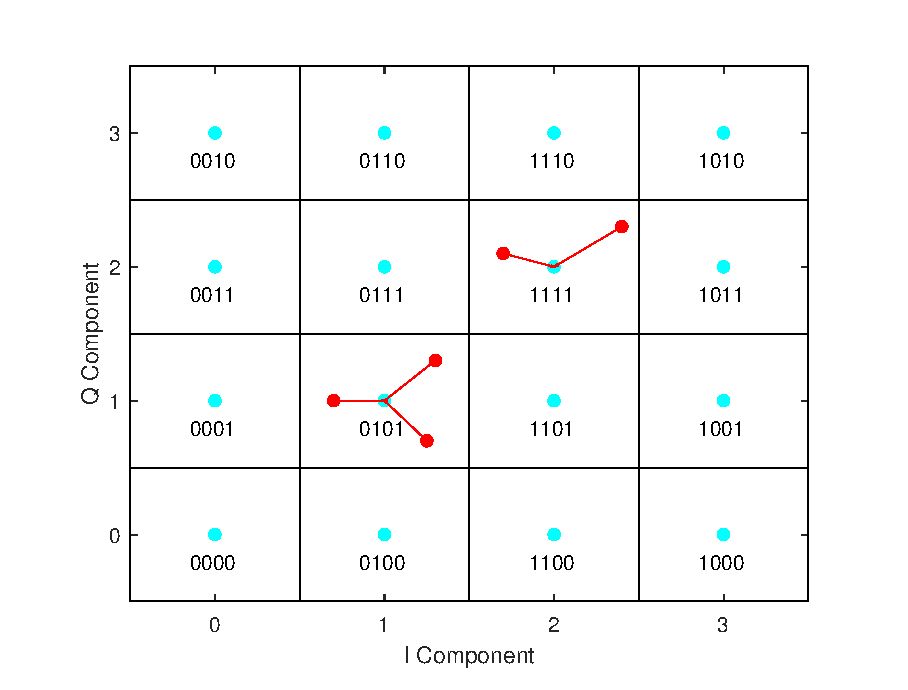
\includegraphics[width=0.7\textwidth]{QAM_Grid.eps}
	\caption{16-QAM constellation with Maximum Likelihood boundaries}
	\label{fig_QAM ML Decoding}
\end{figure}

If the C receiver is successful, the binary file is read into a \textit{NumPy} array to be decoded.
For all modulation schemes, the first step is to de-map the data from the masks to their DAC value(s) using the list \colorbox{backcolour}{\lstinline{DAC_Pins_1}} as well as \colorbox{backcolour}{\lstinline{DAC_Pins_2}} for quadrature-carrier modulation schemes.
The receiver then measures the peak values of the signal and if there has been any attenuation of the signal, it is scaled to the full input range and the attenuation is logged.
PAM and QAM then use Maximum Likelihood (ML) decoding to figure out the correct symbol values.
This equates to using partitions which are halfway between possible symbols to decode them.
For example in 16-QAM, any value within the box around each symbol in Figure \ref{fig_QAM ML Decoding} would be mapped to the symbol at its centre.

\begin{figure}[!h]
 	\centering
 	\includegraphics[width=0.95\textwidth]{Receiver_Flow.png}
 	\caption{Flow Chart for Receiver Code}
 	\label{fig_Receiver_Flow}
\end{figure}

Once the input has been decoded into the ML estimated symbols, it must be recombined into byte-wise data.
For 4PAM this constitutes an OR of the four symbols of a byte, each symbol bit-shifted two bits to the left (multiplied by four) of the next.
For QAM, the mapping table of Listing \ref{lst_Inverted QAM} is inverted and each symbol de-mapped into four bits.
The bits are then packed into 8-bit numbers with the command \colorbox{backcolour}{\lstinline{np.packbits(output_bits)}}.
If the transmission was of an image file, the receiver saves the received data into an image file of the same size, otherwise it saves it to a file where it can be compared to the original data.

\subsubsection{C Transmitter and Receiver} \label{sec_C Transmitter and Receiver}

The C library used for manipulation of the GPIO pins is \textit{pigpio} \cite{lib_pigpio}.
This library uses direct memory access to read the values of the pins, and has functions for reading in or writing to a bank of values as a bitmask.
A bitmask is an unsigned 32-bit integer (in this case) where each bit corresponds to a pin value being '1' or '0'.
The mask uses BCM numbers, and although there are 32 pins which can theoretically be accessed, only BCM pins 2-27 are available for user purposes.
The Python transmitter expands the required DAC bit values (0-7 for 8-bit output) onto the 32-bit mask depending on which GPIO pins the DAC is connected to.
An simplified example of this mask expansion is shown in Figure \ref{fig_Mask Expansion}.
As Section \ref{sec_Advanced Modulation Schemes} explained, an inverted mask is also required to clear the '0'-value bits of their previous values.
Section \ref{sec_Computation} compares the speed of the individual pin read to the bank read operation, and the speed of the individual pin write to a bank set and clear.
In both cases the bank operation is faster - likely because of the direct memory access - as well as reading or setting all required pins at once.
As a result, all of the C code uses these mask operations to set and read the pins.\\

\begin{figure}[ht]
 	\centering
 	\includegraphics[width=0.8\textwidth]{Mask_Expansion.png}
 	\caption{Explanation of the concept of mask expansion}
 	\label{fig_Mask Expansion}
\end{figure}

Another advantage of using bitmasks is that \textit{PiTransmit\textunderscore 3} and \textit{PiReceive} can operate entirely independently of the choice of which GPIOs the DACs and ADCs use, or even whether the modulation scheme is using one or two of each.
The transmitter reads in the array of bitmasks (bits to set) from a binary file, which is calculated and saved in the Python before transmission.
It also reads in the inversion masks (bits to clear) so this calculation is not done during transmission.
The clock pulse goes low with the data and then high \SI{1}{\micro\second} later, going low again at the end of the clock cycle with the next parallel data.
Listing \ref{lst_Transmitter Docs} from the transmitter comments explains the reason for the clock shape.
The transmitter loops through the data masks, bank setting (masks) and clearing (inversion masks) the values for the DAC input and outputting the clock signal, then it closes upon completion.\\

\lstset{style=C}
\begin{lstlisting}[caption={Transmitter documentation explaining the clock signal}, label={lst_Transmitter Docs}, basicstyle=\footnotesize]
	/* Clock cycle will have shape:
	* |_|------------|_|------------|_|------------|_|------------
	* The pulses will be low for 1us ^ and high ^ for the rest of the clock period
	* ADC:
	* Rising _CS_ latches data but read event requires falling then rising edge
	* It holds the output at the latched value until the next falling edge
	* DAC:
	* _WR_ going low clears the converter and _WR_ high starts the conversion
	* _BUSY_ goes high when conversion is complete, and is used as Rx clock pin
	*
	* A 1us pulse is long enough for both converters to use as a trigger (100ns at least)
	* It is also short enough that at max frequency (100kHz) it is still a fraction of
	* a clock pulse	*/
\end{lstlisting}

The receiver starts by allocating a memory block for the number of masks expected.
It then sets up the callback function \colorbox{backcolour}{\lstinline{readPins()}} on the change of state of the clock (ADC $\overline{BUSY}$) pin.
If the event triggered was a rising edge, it saves the value of \colorbox{backcolour}{\lstinline{gpioRead_Bits_0_31()}} into the output array.
A static counter keeps track of the data received, and when it reaches the number of masks expected, closes the callback and changes a global variable \colorbox{backcolour}{\lstinline{pin_state}} to a specific value to signal ending the program.
The callbacks are also closed and this specific value set if there is a watchdog time out -- when the callback is called because there has been no change in the clock pin for a certain amount of time.\\

Once the receiver has set the callbacks on startup, it uses a while loop to wait until the specific exit value is set on \colorbox{backcolour}{\lstinline{pin_state}} to exit the loop and end the program.
Finally, the received bitmasks are saved to a binary file which is opened by the Python code and mapped to ADC pins to decode the received data. 
\end{document}